\chapter{Evaluation}
\label{chapter:evaluation}

Before we evaluate the system, we shall make a few notes that apply to the evaluation of the system as a whole.

\section{Notes}
\label{section:notes}

All the tests and benchmarks were performed on a single machine.
The machine has 16GB of RAM, an M1 Apple Silicon processor 3200 MHz, and a 512GB SSD.
Due to these specs, the benchmarks are run with files between 1MB and 100MB.
We ran benchmarks with files up to 1GB and the results were consistent with the results from the smaller files,
i.e., the algorithms exhibit the same behavior, but rerunning the benchmarks takes a lot of time.

The system is written in Rust, which means no garbage collection or runtime overhead.
We expect very little memory footprint while the system is idle,
which is indeed the case as seen from running 1000 instances in \autoref{fig:1000-instances}.
No CPU usage and around 2MB of memory per instance is used when the system is idle
aligns with our expectations.
Because the system consumes almost no resources when idle,
we can run many instances on a single machine.
We will not account for the overhead of the system being idle in the benchmarks.

\begin{figure}
    \centering
    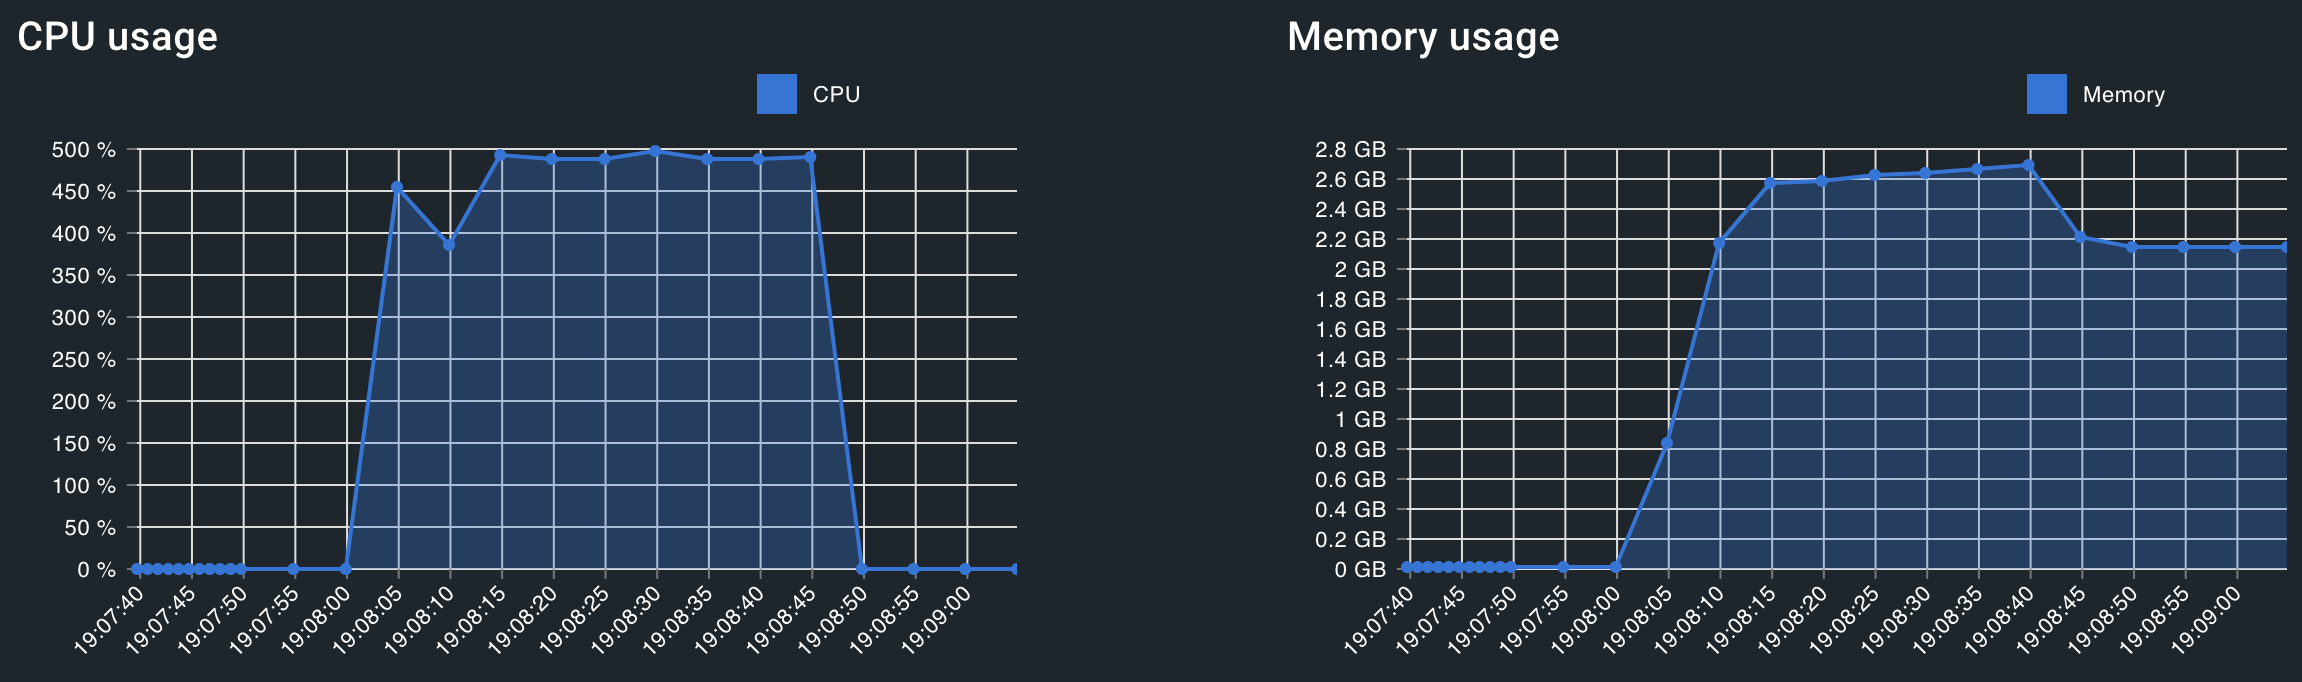
\includegraphics[width=350pt]{gfx/1000-instances.png}
    \captionof{figure}{Starting 1000 instances}
    \label{fig:1000-instances}
\end{figure}

\section{Proof of Retrievability (PoR)}
\label{section:por-evaluation}

In this section, we evaluate how the PoR protocol performs in a real-world scenario.
We have discussed how PoR is used to ensure the integrity of the data stored on the nodes.
Now, we evaluate how viable is it to use PoR as a part of a storage system.
Does it adhere to the \autoref{section:requirements}?
And is it fast enough to be used in a real-world scenario?
The protocol has two parts --- the initial storing of a file and the subsequent repeated audits.

\subsection{Storing a file using PoR}

When storing a file in a distributed system we have to perform some calculations on the data
to generate the metadata required to run the PoR audits later.
This is a one-time operation, which is not crucial to be fast,
but it would provide better user experience if it is.
Ideally the impact should be minimal and proportional to the size of the file,
as seen in \autoref{fig:por-initialize}.

\begin{figure}
  \myfloatalign
  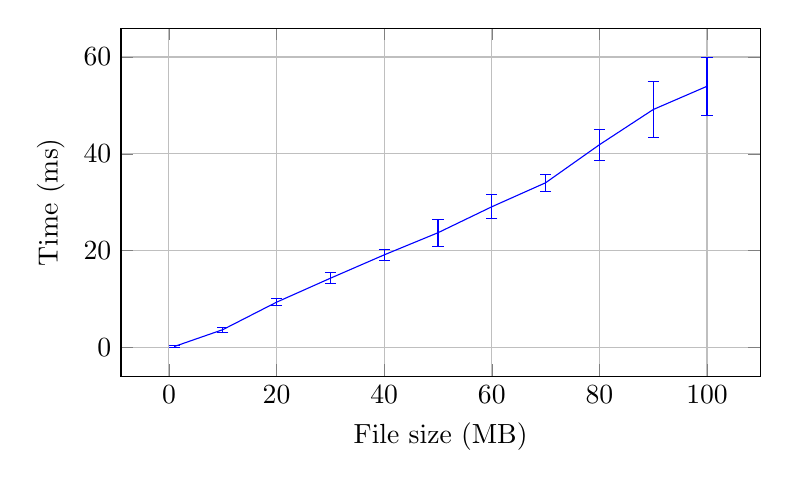
\begin{tikzpicture}
    \begin{axis}[
      xlabel={File size (MB)},
      ylabel={Time (ms)},
      grid=major,
      width=0.8\textwidth,
      height=6cm,
    ]
    \addplot[mark=., blue, error bars/.cd, y dir=both, y explicit] coordinates {
      (1, 0.221311) +- (0, 0.13)
      (10, 3.694679) +- (0, 0.50)
      (20, 9.369777) +- (0, 0.69)
      (30, 14.315975) +- (0, 1.13)
      (40, 19.139883) +- (0, 1.13)
      (50, 23.713537) +- (0, 2.8)
      (60, 29.072395) +- (0, 2.5)
      (70, 34.027716) +- (0, 1.75)
      (80, 41.878575) +- (0, 3.2)
      (90, 49.148558) +- (0, 5.8)
      (100, 53.950145) +- (0, 6.0)
    };
    \end{axis}
  \end{tikzpicture}
  \caption{Time required for the first peer to initialize the metadata for PoR when storing a file.}
  \label{fig:por-initialize}
\end{figure}

\subsection{How many audits can we perform in parallel?}

The audit is a two-step process.
First, the Verifier sends the challenge to the Keeper and then the Keeper responds with the proof.

We expect the load on the Verifier to be negligible, while the load on the Keeper to be significant.
The Verifier should do as little work as possible,
because we want to perform as many audits as possible in parallel.
This way we can ensure that audits are performed often enough to ensure the integrity of the data.
The load on the Keeper is expected to be high,
because the Keeper needs to read the file from disk and execute the PoR algorithm.
Ideally that algorithm will be linear in time complexity in the size of the file.

The Verifier performs 2 operations --- sending the challenge and verifying the proof.
We benchmarked these operations and the results are shown in \autoref{fig:por-verifier-create-challenge}
and \autoref{fig:por-verifier-audit-challenge}.

The results show that generating the challenge and auditing are both very fast operations ---
for a 100MB file, the Verifier can generate the challenge in 0.027ms and
audit the proof in 0.137ms.

We can observe something interesting the in the results ---
the graph looks almost logarithmic, instead of linear.
This is due to cache locality since both the operations are executing code on sequential memory addresses.
Both the challenge and the response are essentially a vector of numbers,
which is a very cache-friendly data structure.

\begin{figure}
  \myfloatalign
  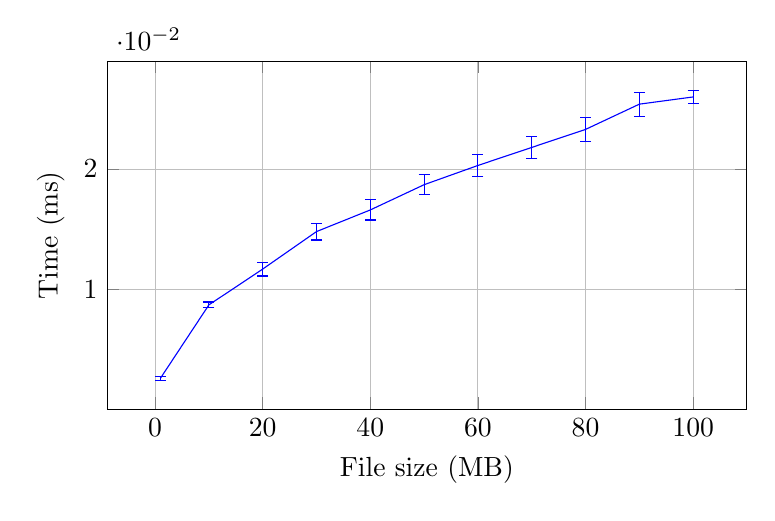
\begin{tikzpicture}
    \begin{axis}[
      xlabel={File size (MB)},
      ylabel={Time (ms)},
      grid=major,
      width=0.8\textwidth,
      height=6cm,
    ]
    \addplot[mark=., blue, error bars/.cd, y dir=both, y explicit] coordinates {
      (1, 0.0026) +- (0, 0.000157)
      (10, 0.0087) +- (0, 0.000237)
      (20, 0.01168) +- (0, 0.000577)
      (30, 0.0148) +- (0, 0.000699)
      (40, 0.0166) +- (0, 0.000833)
      (50, 0.0187) +- (0, 0.000850)
      (60, 0.0203) +- (0, 0.000891)
      (70, 0.0218) +- (0, 0.000917)
      (80, 0.0233) +- (0, 0.001)
      (90, 0.0254) +- (0, 0.001)
      (100, 0.026) +- (0, 0.000562)
    };
    \end{axis}
  \end{tikzpicture}
  \caption{Time required for the Verifier to create the challenge for PoR.}
  \label{fig:por-verifier-create-challenge}
\end{figure}

\begin{figure}
  \myfloatalign
  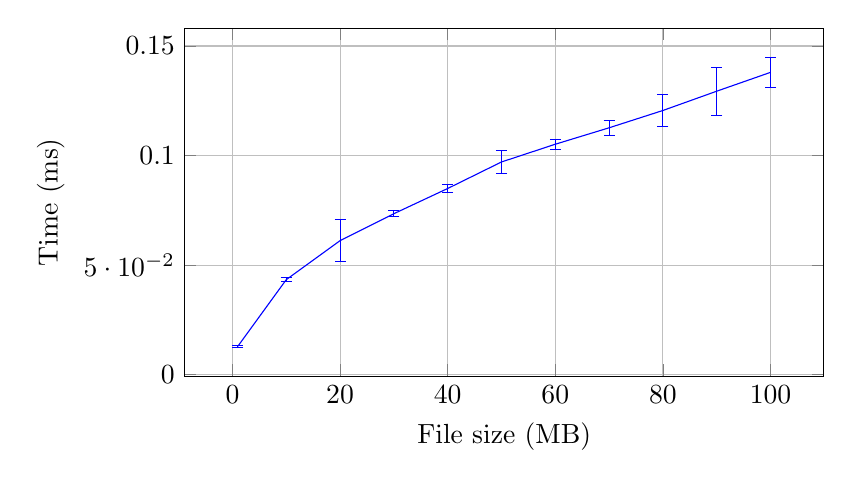
\begin{tikzpicture}
    \begin{axis}[
      xlabel={File size (MB)},
      ylabel={Time (ms)},
      grid=major,
      width=0.8\textwidth,
      height=6cm,
    ]
    \addplot[mark=., blue, error bars/.cd, y dir=both, y explicit] coordinates {
      (1, 0.013) +- (0, 0.000396)
      (10, 0.0434) +- (0, 0.000971)
      (20, 0.0612) +- (0, 0.00956)
      (30, 0.0735) +- (0, 0.00135)
      (40, 0.0850) +- (0, 0.0017)
      (50, 0.0971) +- (0, 0.0051)
      (60, 0.1052) +- (0, 0.0023)
      (70, 0.1127) +- (0, 0.00343)
      (80, 0.1206) +- (0, 0.0074)
      (90, 0.1294) +- (0, 0.0109)
      (100, 0.138) +- (0, 0.0069)
    };
    \end{axis}
  \end{tikzpicture}
  \caption{Time required for the Verifier to audit the challenge response PoR.}
  \label{fig:por-verifier-audit-challenge}
\end{figure}

The Keeper performs 1 operation --- generating the proof.
This is done by reading the file from disk and running the PoR algorithm on it.
The PoR algorithm is expected to be linear in time complexity in the size of the file.
We benchmarked this operation and the results are shown in \autoref{fig:por-keeper-challenge-generate}.

The operation gets slower as the file size increases.
In theory the time complexity should be linear, but it is superlinear in practice.
This is most likely caused by the unoptimized matrix multiplication algorithm that we are using to
implement PoR.

\begin{figure}
  \myfloatalign
  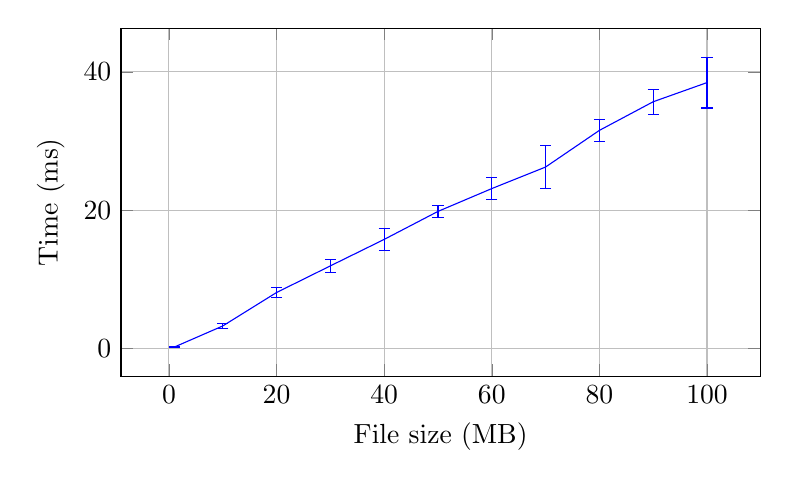
\begin{tikzpicture}
    \begin{axis}[
      xlabel={File size (MB)},
      ylabel={Time (ms)},
      grid=major,
      width=0.8\textwidth,
      height=6cm,
    ]
    \addplot[mark=., blue, error bars/.cd, y dir=both, y explicit] coordinates {
      (1, 0.21) +- (0, 0.01)
      (10, 3.26) +- (0, 0.42)
      (20, 8.1) +- (0, 0.74)
      (30, 11.95) +- (0, 0.93)
      (40, 15.78) +- (0, 1.56)
      (50, 19.83) +- (0, 0.86)
      (60, 23.13) +- (0, 1.62)
      (70, 26.25) +- (0, 3.13)
      (80, 31.55) +- (0, 1.6)
      (90, 35.69) +- (0, 1.8)
      (100,38.46) +- (0, 3.67)
    };
    \end{axis}
  \end{tikzpicture}
  \caption{Time required to create the challenge response (proof) for PoR on the Keeper side, without reading the file from disk.}
  \label{fig:por-keeper-challenge-generate}
\end{figure}

\subsection{Is PoR the limiting factor in the system?}

One of the main questions we want to answer in this thesis is whether the validation component
affects the system's performance.
From the results we can see that while the evaluation aspect introduces more workload,
however, it is within reasonable levels.

In the previous section we saw that the Verifier can generate the challenge and audit the proof very quickly.
Since the speed of reading from an SSD is on average 7000 MB/s, the PoR protocol in the Verifier
will not affect the system's performance.
It is more likely, that the network connection between the Verifier and the Ledger will be the limiting factor,
but we will not evaluate network speeds as they are out of the scope of this thesis.

The Keeper can generate the proof at a rate of 38ms for a 100 MB.
This is faster than the access speed of an HDD, which is around 500 MB/s or 200ms for a 100 MB.
However, it is slower than the access speed of an SSD, which is around 7000 MB/s or 14ms for a 100 MB.
Whether the PoR protocol is the limiting factor or not depends on what kind of storage the Keeper is using.

In conclusion, the Verifier can send challenges in parallel, but the Keeper nodes will still be
the limiting factor in the system.

\section{Performance of the system}

Our final goal is to augment a distributed storage system with verification based on PoR.
In the process we want to ensure that the performance of the system is not degraded.
The main part we are changing is the way files are stored, by injecting the PoR initialization,
and the idle state of the peers --- during which they perform audits.
We performed the benchmarks starting with 10 and up to 100 peers in the network.
Since the tests are run on a single machine, running more peers would not give us any useful information,
because the resources of the machine will be exhausted from running the peers in idle state.
This is also the reason we are using files of size up to 10MB.
Larger files would take more time to read and write to disk,
but would not give us any additional information about the performance of the system.

From \autoref{table:storage} we can see the overhead of running the PoR algorithm and
writing the metadata to the ledger.
It takes six to 10 times longer for the storage request to be processed
in comparison to running only the base Kademlia.
While our implementation is not optimized and processes the requests sequentially,
we can see that the overhead is significant.
We run PoR separately for each replica that is to be stored.
We would have expected two to three times longer processing time,
not six times longer.
The main cause for this is the ledger.
Sending requests to the ledger is sequential and while the ledger has high throughput,
a lot of requests tend to fail.
A lot of times when we send a request to the ledger, it would fail because the state has changed.
This is not something documented in the Immudb's documentation, but to circumvent it,
we are retrying the requests until they succeed, which is usually on the second or third try.

Despite the overhead, storing a file is a one time operation,
so while we can improve it, it is not a critical issue.

\subsection{Running a Verifier and a Keeper separately or together}

The final goal is for each peer in the system to run one binary,
that is both a Keeper and a Verifier.
However, our implementation is not highly parallelized,
so we expect that running the Keeper and Verifier separately will be faster.

The results of the benchmarks are once again in \autoref{table:storage}.

It is important to note that having 10 or 100 nodes in the network does not seem to impact the
time to store files.
This is the case because before running each benchmark we wait for the peers in the network
to connect to each other.
We do not run the tests immediately after a cold start of the system.

The Time without Verifier from \autoref{table:storage} is when the node that accepts the storage request
does not run the Verifier, and the Time with Verifier is when the node runs the Verifier as well.
The time to process a request with the Verifier running is significantly longer.
This is mainly due to the outlier requests, which have to be processed while a verification is running.
The longest request time column shows the extreme outliers,
with the standard deviation showing how much the requests vary.
With our current architecture, the ledger module and the Kademlia swarm module are both singleton modules,
locked behind mutexes, to ensure that no race conditions occur.
This causes the Verifier to occasionally take a hold of these mutexes and block the
storage requests from being processed.
This can be circumvented by running a pool of connections to the ledger and the swarm.
We have left this for future work as it can be circumvented by each peer running 2 nodes ---
one for storage and one for verification.

\begin{landscape}
  \begin{table}[h]
    \centering
    \myfloatalign
    \pgfplotstabletypeset[
    col sep=comma,
    every head row/.style={ before row=\toprule, after row=\midrule },
    every last row/.style={ after row=\bottomrule },
    columns={npeers, data, kad, time, timever, p99},
    columns/npeers/.style={string type, column name=\shortstack{\textsc{Number} \\ \textsc{of peers}}, dec sep align, fixed },
    columns/data/.style={ column name=\shortstack{\textsc{Data} \\ \textsc{stored}}, column type=r, string type},
    columns/kad/.style={ column name=\shortstack{\textsc{Kademlia}}, string type, column type=r},
    columns/time/.style={ column name=\shortstack{\textsc{Time without} \\ \textsc{Verifier}}, string type, column type={r}},
    columns/timever/.style={ column name=\shortstack{\textsc{Time with} \\ \textsc{Verifier}}, string type, column type=r},
    columns/p99/.style={ column name=\shortstack{\textsc{Longest} \\ \textsc{request time}}, string type, column type=r},
    columns/stddev/.style={ column name=\shortstack{\textsc{Standard} \\ \textsc{deviation}}, string type, column type=r},
    ]{./data/store.csv}
    \caption{Storing files in the system with replication factor of 3. Each benchmark is ran 100 times. Longest request time and Standard deviation both refer to the column for Time with Verifier.}
    \label{table:storage}
  \end{table}
\end{landscape}

\section{How fast are malicious behaviors detected?}

We are interested in how fast the system can detect a malicious peer.
We define detecting a malicious peer by the time it takes for the system to find the first
sign of misbehaving.
The faster a malicious peer is detected, the faster the system can react to it.
We expect with the increase of files in the system or increase of peers, the time to
detect a malicious peer to decrease.

\subsection{Detecting a malicious Keeper}

For Keepers, the malicious behavior is corrupting data.
We expect with the increase of files in the system, the time to detect a malicious Keeper to decrease.

All files are verified each cycle in our testing environment.
In a real world scenario, this is achievable only with very long cycles.
The alternative option is to check a random subset of the files each cycle,
which will provide probabilistic guarantees that a malicious Keeper will be detected.

The Verifiers split the work of verifying the files based on the file's key.
As an example, if we have two peers (2 Keepers and 2 Verifiers),
the Verifiers would split the files of each Keeper and take turns verifying them
during alternating cycles.
This is illustrated in \autoref{fig:2-verifiers}.

\begin{figure}
    \centering
    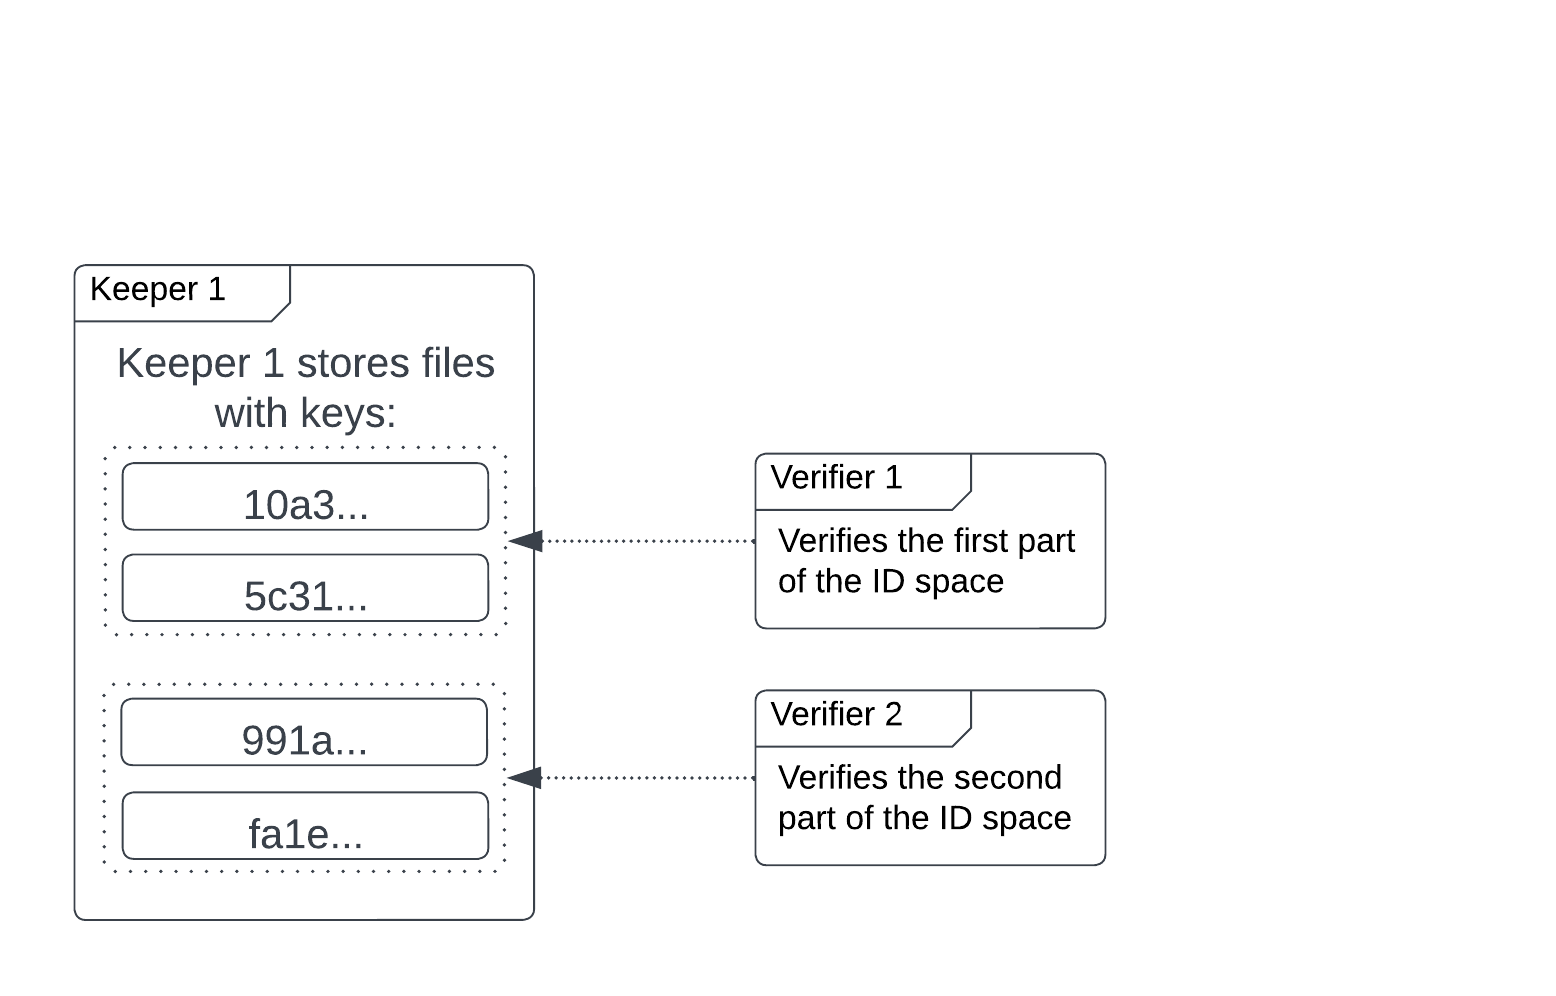
\includegraphics[width=350pt]{gfx/2-verifiers.png}
    \captionof{figure}{Splitting the ID space between two Verifiers}
    \label{fig:2-verifiers}
\end{figure}

This means that when a peer becomes malicious they have at most one cycle of time,
before they are detected.
We are running the benchmarks in \autoref{table:verify_detection_times} with various amount of data in the system.
The cycle times are chosen arbitrarily in order to provide an overview of how the system behaves with
different cycle times and to show the connection between the amount of data and the cycle length.
The cycle time when running the system in production should be set to a value proportional to
the amount of data and number of files stored in the network.
We are running the benchmarks with 1 corrupt peer in the network,
because if we have more the chance of a corrupt peer being detected increases.
We are interested in how long it takes to discover the first signs of misbehaving in the network.
The general observation, which is not surprising, is that the more files we have in the network,
the faster it is to discover a corrupt peer,
because the greater the chance it is for the corrupt peer to store a file.
For example, with 100 peers and 100 files in the system, the corrupt peer is expected to store 1 file,
That means that all the files need to be verified in order to discover the corrupt peer.
This is even more apparent with 10 peers where the time to discover a corrupt peer with 1000 files is
41ms in comparison with 1120ms for 100 files.

\subsection{Detecting a malicious Verifier}

For Verifiers, the malicious behavior is not performing audits.
We expect with the increase of files in the system, the time to detect a malicious Verifier to decrease.
Detecting a malicious Verifier is very similar to detecting a malicious Keeper,
and we could show similar results for the minimum times required to detect a malicious Keeper.
Instead, we would like to confirm that a malicious Verifier will be detected in a reasonable time.
Reasonable time is within two cycles, because the Verifiers are expected to perform audits every cycle.

The results are shown in \autoref{table:verify_averages}.
The average time to detect a malicious Verifier indeed remains within two cycles.
There is no significance in the actual time - the difference between 2000ms and 5000ms average is not
meaningful, as it depends on what time the peer initiates the auditing cycle.
The peers do not have synchronized clocks, so one peer's cycle might just start 3000ms later than the other.
Again, at 50 peers or more the hardware becomes overloaded and starts affecting the times to detect 
malicious Verifiers.
This is expected, mainly because of the communication overhead between the peers.

\begin{table}
  \centering
  \pgfplotstabletypeset[
    col sep=comma,
    every head row/.style={before row=\toprule, after row=\midrule},
    every last row/.style={after row=\bottomrule},
    columns={npeers, data, cycle_time, avg, stddev},
    columns/npeers/.style={string type, column name=\shortstack{\textsc{Number} \\ \textsc{of peers}}},
    columns/data/.style={column name=\shortstack{\textsc{Data} \\ \textsc{stored}}, column type={r}, string type},
    columns/cycle_time/.style={column name=\shortstack{\textsc{Time per} \\ \textsc{cycle}}, string type, column type={r}},
    columns/avg/.style={column name=\shortstack{\textsc{Average} \\ \textsc{time}}, string type, column type={r}},
    columns/stddev/.style={column name=\shortstack{\textsc{Standard} \\ \textsc{deviation}}, string type, column type={r}}
  ]{./data/verify_verifier.csv}
  \caption{Time to discover a corrupt Verifier in the network with 1 corrupt Verifier}
  \label{table:verify_averages}
\end{table}

We are downsizing the tests to only run with 100 files in the system with six seconds cycle time.
Performing so many verifications requires longer cycle times, otherwise the Verifiers start lagging
behind, and we see increasing times to detect malicious peers as seen in \autoref{fig:increasing}.

To deal with this, if we want to add more files to the system we would have to increase the
cycle time, or increase the number of Verifiers.

\begin{figure}
  \centering
  \begin{tikzpicture}
    \begin{axis}[
      xlabel={Index},
      ylabel={Time (ms)},
      grid=major,
      width=0.8\textwidth,
      height=8cm,
    ]
    \pgfplotstableread[col sep=comma]{./data/increasing.csv}\datatable
    \addplot[mark=., blue] table [x expr=\coordindex+1, y=time] {\datatable};
    \end{axis}
  \end{tikzpicture}
  \caption{With too many files and short cycle times, the time to detect a malicious peer increases as the
  Verifiers start lagging behind}
  \label{fig:increasing}
\end{figure}

\subsection{Are the minimum times to detect a malicious peer reasonable?}

During our benchmarks we are assuming that the malicious peers are partially well-behaved.
In particular, they would not try to predict when the Verifier would audit their files.
Under a real attack, that would not be the case.
The malicious peer could record the time between audits and then only come online during the next audit cycle.
If there are not too many files in the system, during an audit cycle, all the audits would be performed
at the beginning and then there would be a downtime until the next cycle.
During this downtime the malicious peer could go offline and save resources, making the
files unavailable but still passing the audits.

To mitigate this, the Verifier could also record how much time all the audits during a cycle take
and then either:
\begin{enumerate}
  \item Run a consensus algorithm with the other peers in order to shorten the cycle time. ---
    This would increase the load on the system and make the audits more common, but lead to increased security.
  \item Randomize the time and order in which audits are performed. --- This would make it impossible for the
    malicious peer to predict when the audits are performed, but it has a probabilistic nature. We are not
    guaranteed to catch the malicious peer immediately after it becomes malicious, but statistically,
    after enough cycles it will be caught.
\end{enumerate}

Both of these options are viable and depend on the requirements of the users of the system.
If the users require a higher level of security and can spare the resources,
the first option is better.
However, if the users want to save resources they could opt for the second approach.
We are not running the benchmarks with these options, because we are mainly interested in
showing that the system can detect malicious behaviors in reasonable time if given the right parameters
and resources.
The analysis of the relation between the length of the verification cycle, the size of the data in the system,
and how they affect the time to detect malicious behaviors, is left for future work.

\subsection{Hardware limitations for the tests}

In \autoref{section:notes} we discussed that the benchmarks are run on a single machine,
and that we can run 1000 instances of the system.
However, this is if we run them idle.
If we run all the instances with enabled storage and verification, i.e., full load,
we see degrading performance with more than 30 instances.
In \autoref{table:verify_detection_times} we can see that for 10 and 20 peers,
the results are consistent, but with 30 peers and with 50, the time to detect a peer is significantly longer.
This is because the hardware becomes overloaded.

In conclusion, with sufficient hardware the system detects malicious peers when the number of peers
increases and the number of files stored in the network increases.
However, if the peers become overloaded, the time to detect a malicious peer increases.

\begin{table}
  \myfloatalign
  \pgfplotstabletypeset[
  every head row/.style={ before row=\toprule, after row=\midrule },
  every last row/.style={ after row=\bottomrule },
  columns={npeers, data, cycle_time, time},
  columns/npeers/.style={string type, column name=\shortstack{\textsc{Number} \\ \textsc{of peers}}},
  columns/data/.style={ column name=\shortstack{\textsc{Data} \\ \textsc{stored}}, column type=r, string type},
  columns/cycle_time/.style={ column name=\shortstack{\textsc{Time per} \\ \textsc{cycle}}, string type, column type={r}},
  columns/time/.style={ column name=\shortstack{\textsc{Time to discover} \\ \textsc{corrupt peer}}, string type, column type=r},
  ]{./data/verify.csv}
  \caption{Time to discover a corrupt peer in the network with 1 corrupt peer}
  \label{table:verify_detection_times}
\end{table}

% 10      100x1KB     60s           20386ms
% 10      1000x1KB    60s           107ms
% 20      100x1KB     60s           2221ms
% 20      1000x1KB    60s           82ms

\section{Reputation system based on a ledger}

The results of the PoR are stored in a ledger, which acts as the source of truth for
the performance of the peers in the network.
While ideally we would like to have a decentralized ledger, for the sake of simplicity
we will use a centralized ledger in our evaluation.
For the purposes of evaluation we could have used a simple SQL database or a local file,
however, we used Immudb because it is what we used in the previous iterations of the system
and at the time we were exploring it as a potential solution for the ledger.
Immudb turned out to have a lot of limitations and we would not recommend it for a production storage system,
such as the one described in this thesis.

\subsection{How does a ledger contribute to the system?}

Using PoR allows peers to detect other peers, which are disrupting the integrity of the data in the system.
However, on its own, it is not enough to ensure that malicious peers are detected and removed from the network.

Is a reputation system based on a ledger a viable measure against malicious nodes?
We expect the ledger to be the source of truth for the reputation of peers and allow
each peer to fetch said reputation and adjust its behavior accordingly.

In \autoref{fig:reputation_loss} we can see how the reputation of a peer changes after it becomes malicious.
All peers in the network start with the same neutral reputation, which is 0.
After 60 seconds, that is 10 cycles, one peer becomes malicious and corrupts some percentage of the data.
The reputation of the peer starts to decrease and goes into the negatives.
Once the reputation drops below 0, the peer is seen as malicious by the other peers in the network,
and can be removed from the network.
This example is for a very short period of time, but in a real-world scenario, the trends will be the same,
just over a longer period of time --- malicious peers would lose reputation --- the more data they corrupt,
the faster they lose reputation.

\begin{figure}
  \centering
  \begin{tikzpicture}
    \begin{axis}[
      xlabel={Time (s)},
      ylabel={Reputation},
      grid=major,
      width=0.8\textwidth,
      height=8cm,
      legend pos=outer north east,
      cycle list name=color list,
    ]

    % Read the data from the CSV file
    \pgfplotstableread[col sep=comma]{./data/rep.csv}\datatable

    % Manually specify legend entries and colors
    \addplot[mark=none, thick, color=blue] table [x expr=\coordindex, y index=0] {\datatable};
    \addlegendentry{0\% corrupted files}

    \addplot[mark=none, thick, color=cyan] table [x expr=\coordindex, y index=1] {\datatable};
    \addlegendentry{10\% corrupted files}

    \addplot[mark=none, thick, color=green] table [x expr=\coordindex, y index=2] {\datatable};
    \addlegendentry{20\% corrupted files}

    \addplot[mark=none, thick, color=lime] table [x expr=\coordindex, y index=3] {\datatable};
    \addlegendentry{30\% corrupted files}

    \addplot[mark=none, thick, color=yellow] table [x expr=\coordindex, y index=4] {\datatable};
    \addlegendentry{40\% corrupted files}

    \addplot[mark=none, thick, color=orange] table [x expr=\coordindex, y index=5] {\datatable};
    \addlegendentry{50\% corrupted files}

    \addplot[mark=none, thick, color=red] table [x expr=\coordindex, y index=6] {\datatable};
    \addlegendentry{60\% corrupted files}

    \addplot[mark=none, thick, color=magenta] table [x expr=\coordindex, y index=7] {\datatable};
    \addlegendentry{70\% corrupted files}

    \addplot[mark=none, thick, color=purple] table [x expr=\coordindex, y index=8] {\datatable};
    \addlegendentry{80\% corrupted files}

    \addplot[mark=none, thick, color=brown] table [x expr=\coordindex, y index=9] {\datatable};
    \addlegendentry{90\% corrupted files}

    \addplot[mark=none, thick, color=black] table [x expr=\coordindex, y index=10] {\datatable};
    \addlegendentry{100\% corrupted files}

    % Draw a horizontal line at y=0
    \addplot[black, thick] coordinates {(0,0) (100,0)};

    % Draw a vertical line at x=60 with text
    \draw[red, thick, dashed] (axis cs:60,-70) -- (axis cs:60,60) node[pos=1, above] {Peer becomes malicious};

    \end{axis}
  \end{tikzpicture}
  \caption{Reputation loss over time for different percentages of corrupted data.}
  \label{fig:reputation_loss}
\end{figure}

% I'm still playing around with this idea, I'm not sure if this is the best way to do it.
% Perhaps the staked reputation will be returned gradually with each successful audit.
% The whole idea of adding "staking" is to ensure the peer has a big hit in reputation from the beginning.
% This way a new peer in the network cannot just accept a lot of files as soon as it joins and then go offline.}
% Every time an audit is performed the reputation of the peer on which the audit was performed is adjusted.
% If the audit is successful, the reputation of the peer is increased,
% and if the audit fails, the reputation of the peer is decreased.
% Finally, a peer is awarded reputation points for performing audits.
% The increase and decrease numbers are configurable and can be adjusted to fit the network requirements.
% We will discuss the different possibilities for adjusting the reputation in the \autoref{chapter:evaluation}

% We need to answer the question of how often audits should be performed and how often nodes should
% check the audit results of others.
% The overhead of performing audits should be as low as possible, but the audits should be performed often enough
% to ensure the integrity of the data.

% Finding the balance between audits and the overhead of the audits, and the penalties and rewards for the nodes
% is crucial for the success of the system.
% We will evaluate the system by running it with different parameters and observing the behavior of the nodes.
% We will discuss the details and the results of the evaluation in \ref{chapter:evaluation}.

\section{Balancing the reputation system}

% We need to evaluate the proper penalties and rewards for the nodes.
% A good balance is needed between rewards and penalties to ensure that a node is
% going to perform enough work for the system before being able to harm it.
% Part of this evaluation will be:
% \begin{enumerate}
%     \item How much reputation points a node stakes when it stores a file?
%     \item How much reputation points a node loses when it fails an audit?
%     \item How much reputation points a node gains when it performs an audit?
%     \item How much reputation points a node loses when it's discovered to not be performing audits?
%     \item What is the starting reputation for new nodes?
%     \item How do nodes increase their reputation at the very beginning?
%     \item Does having high reputation give the node any benefits?
% \end{enumerate}

% Nodes with very high reputation could easily become malicious as they can absorb the penalties.
% We need to solve this problem by either having a maximum reputation or by having the penalties be
% percentage-based.

One of the main questions we want to answer in this thesis is
how to balance the reputation once we have PoR and the ledger in place.

The reputation is controlled by two parameters:
\begin{enumerate}
  \item Reputation increase for storing a file or performing an audit.
  \item Reputation decrease for corrupting data or not performing audits.
\end{enumerate}

We need to find the right balance between the two.
If the reputation increase is too high, the nodes can easily become malicious,
as they can absorb the penalties.
If the reputation decrease is too high, the nodes will not be able to recover from a mistake,
such as being temporarily offline or being under heavy load for a period of time.

\subsection{Balancing the reputation gain/loss}
\label{section:balancing}

The reputation gain and loss are parameters of the system that can be adjusted.
For our evaluation we are using the following parameters:
\begin{itemize}
  \item Reputation increase for storing a file: 1
  \item Reputation increase for performing an audit: 1
  \item Reputation decrease for corrupting data: 5
  \item Reputation decrease for not performing an audit: 5
\end{itemize}

These numbers are arbitrary, and the only important thing is that the reward is 20\% of the penalty.
In such a configuration we expect that:
\begin{itemize}
  \item Peers that fail less than 20\% of the time to keep gaining reputation slowly.
  \item Peers that fail 20\% of the time to maintain their reputation.
  \item Peers that fail more than 20\% of the time to slowly lose reputation.
\end{itemize}

We ran the benchmark similarly to the previous benchmarks --- 
1 peer goes malicious after 60 seconds and corrupts some percent of the data.
The results are shown in \autoref{fig:reputation_loss_selected}.
The benchmarks this time are run for 300 seconds, because we want to observe the long-term trends,
unlike \autoref{fig:reputation_loss} where we were interested in how the extreme cases compare.

As predicted when the reward is 20\% of the penalty, a peer that is corrupting 10\% of the data
slowly increases its reputation, a peer that is corrupting 20\% of the data maintains its reputation,
and a peer that is corrupting 30\% of the data slowly loses reputation.
There are some oscillations in the data, which is due to the cycle time and what are the file IDs,
that are being corrupted.

\begin{figure}
  \centering
  \begin{tikzpicture}
    \begin{axis}[
      xlabel={Time (s)},
      ylabel={Reputation},
      grid=major,
      width=0.8\textwidth,
      height=8cm,
      legend pos=outer north east,
    ]

    % Read the data from the CSV file
    \pgfplotstableread[col sep=comma]{./data/rep300.csv}\datatable

    \addplot[mark=none, thick, color=blue] table [x expr=\coordindex, y index=0] {\datatable};
    \addlegendentry{10\% files are corrupted}

    \addplot[mark=none, thick, color=black] table [x expr=\coordindex, y index=1] {\datatable};
    \addlegendentry{20\% files are corrupted}

    \addplot[mark=none, thick, color=red] table [x expr=\coordindex, y index=2] {\datatable};
    \addlegendentry{30\% files are corrupted}

    % Draw a horizontal line at y=0
    \addplot[black, thick] coordinates {(0,0) (300,0)};

    % Draw a vertical line at x=60 with text
    \draw[red, thick, dashed] (axis cs:60,-70) -- (axis cs:60,60) node[pos=1, above] {Peer becomes malicious};

    \end{axis}
  \end{tikzpicture}
  \caption{Reputation loss over time for 10\%, 20\%, and 30\% corrupted data.}
  \label{fig:reputation_loss_selected}
\end{figure}

The conclusion we can derive from this experiment is that the leeway we give to peers is customizable,
based on what the user requirements are.
If we wish to have a very strict system and allow only 5\% leeway (corrupted data or peers being offline),
we can set the reward to be 5\% of the penalty.
On the other hand, if we know the peers are going to be going offline for 8 hours each day,
because the users turn off their computers at night, we can set the reward to be greater than 33.3\% of the penalty.

\subsection{Recovering reputation}

It is possible for a peer to have downtime.
Perhaps the network was disturbed, or the peer had to be restarted for updates.
In such cases, the peer would lose reputation, which it can recover if it behaves well afterwards.

The time that a peer can be offline should depend on its contribution thus far.
Since we treat going offline as failing all audits, this is not much different from a peer
behaving maliciously for a short period of time.
The main thing we want to see is that a peer can recover its reputation after failing a few audits,
as long as it is above the threshold of being removed from the network (zero reputation).

We ran a simulation with a peer that goes offline for two cycles and then for one cycle.
The reward in our simulation is 20\% of the penalty.
The results are shown in \autoref{fig:reputation_recovery}.
From the results we can see that the peer's reputation starts dropping shortly after it goes offline.
The exact time depends on when the next audit will happen, but is within the one cycle range.
Since the peer does not drop below zero reputation, after coming back online, it starts recovering its
reputation, which is exactly what we want to see.
There are no long-term effects of going offline for a short period of time.

As a conclusion, a peer can go offline for a short period of time and recover its reputation afterwards,
as long as it has contributed to the network sufficiently before going offline.
How long a peer can go offline depends on the configuration of the reputation adjustments,
similarly to the previous section.
If we configure the increase of reputation for succeeding audits to be ten times less than the decrease
for failing audits, the peer can go offline for 10\% of the time and maintain its reputation.

\begin{figure}
  \centering
  \begin{tikzpicture}
    \begin{axis}[
      xlabel={Time (s)},
      ylabel={Reputation},
      grid=major,
      width=0.8\textwidth,
      height=8cm,
    ]
    \pgfplotstableread[col sep=comma]{./data/recovery.csv}\datatable
    \addplot[mark=none, blue] table [x expr=\coordindex, y=reputation] {\datatable};
    \addplot[black, thick] coordinates {(0,0) (294,0)}; % Draws a horizontal line at y=0
    \draw[red, thick, dashed] (axis cs:96,0) -- (axis cs:100,60) node[pos=1, above] {Peer goes offline for 2 cycles};
    \draw[red, thick, dashed] (axis cs:190,50) -- (axis cs:185,0) node[pos=1, above] {Peer goes offline for 1 cycle};
    \end{axis}
  \end{tikzpicture}
  \caption{Reputation of a peer, which goes offline twice for two and for one cycles respectively.}
  \label{fig:reputation_recovery}
\end{figure}

\section{Using Rust}

Rust is a systems programming language that is known for its performance and safety.
For these reasons we chose it for this project.

Rust provides thread safety and memory safety without a garbage collector.
Since the system is multithreaded, and it is composed of different modules
that communicate with each other, Rust forces us to use mutexes or channels
to communicate between threads.
Without them, the compiler would not allow us to compile the code.
We also get no memory leaks, as Rust has a strict ownership model.
It is also a well-rounded language, with a lot of libraries and frameworks available,
which makes it a good choice for a project like this.
Also, because of the small memory footprint of the system and the low CPU usage,
we can run many instances of the system on a single machine,
allowing us to test the system with many peers.

While the pros of using Rust are many, there are some cons as well.
In particular, the learning curve of Rust is steep and takes time to get used to
the different coding style.
Even after being comfortable with the language, it takes longer to develop in Rust
because of the strict compiler rules and explicitness of the language.
Running benchmarks is a difficult task as they are not fully supported ---
we have to use either external libraries or unstable features of the language.

Overall, Rust is a good choice for a project like this, because of its safety and performance,
but the extra time to develop in Rust should be taken into account.

\section{Summary}

It is difficult for storage system with potential malicious nodes to compete
head-to-head with centralized cloud storage providers, which optimize every aspect of their system.
Introducing Proof of Retrievability (PoR) into the system brings us closer to the guarantees
that cloud storage providers offer.
This is not without its costs, as we have seen in the evaluation --- any additional work
that the nodes have to perform will increase the time to process requests.
It is an unavoidable trade-off between security and performance.
However, the performance overhead of PoR is not so significant if we take into account that
cloud services also perform integrity checks on the data stored on their servers,
albeit with slightly lighter algorithms.
The main bottleneck is the ledger, which in our tests is centralized.
Even if it has high advertised throughput, under load, especially with a lot of data,
and the many failed requests, it becomes a bottleneck.
For PoR to be a viable solution for a storage system, the ledger has to be decentralized as well.
